\begin{figure}[htbp]
    \centering
    \begingroup
    \scriptsize
    \setlength{\tabcolsep}{2pt}
    \resizebox{\textwidth}{!}{%
    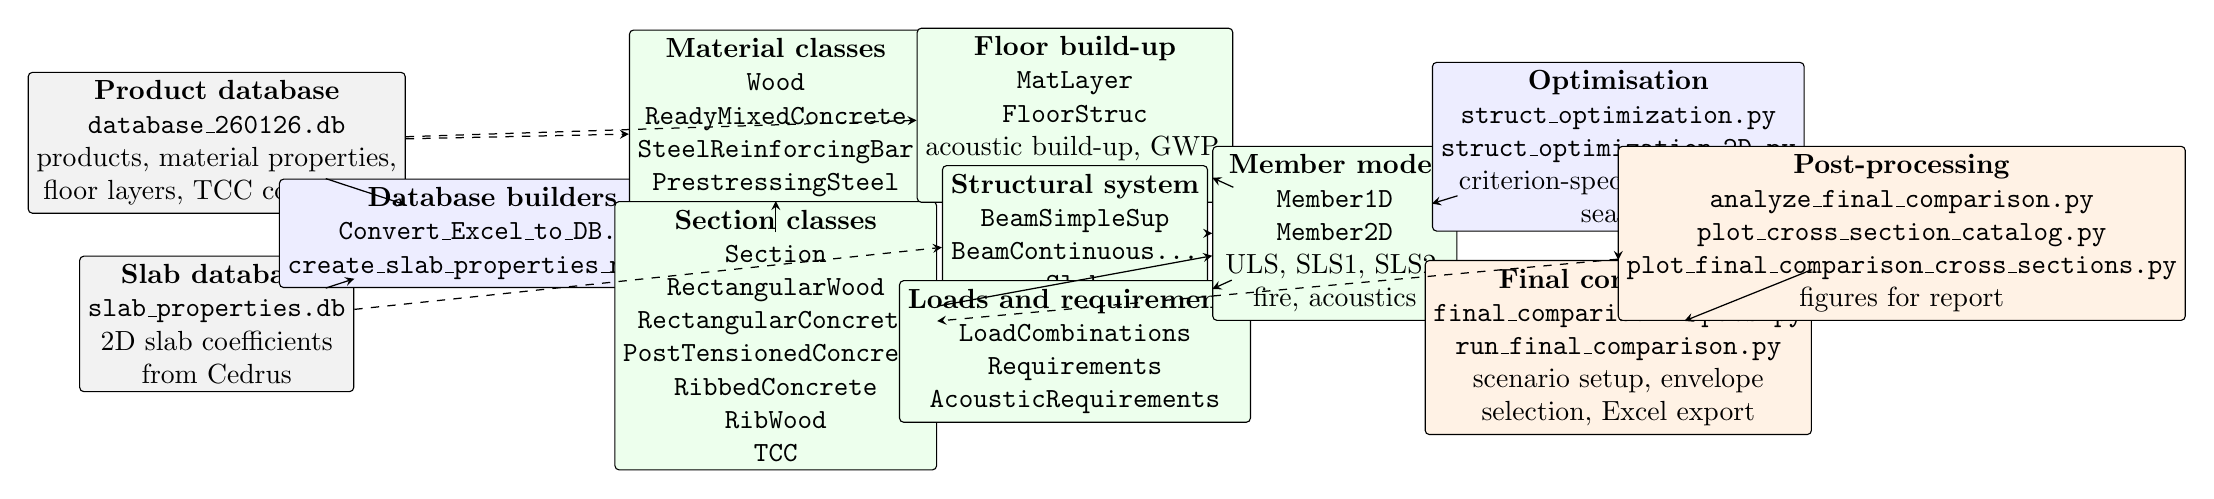
\begin{tikzpicture}[
        >=stealth,
        box/.style={draw, rounded corners=1.5pt, align=center, minimum width=31mm, minimum height=8mm, inner sep=3pt},
        module/.style={box, fill=blue!7},
        class/.style={box, fill=green!7},
        data/.style={box, fill=gray!10},
        final/.style={box, fill=orange!10},
        rel/.style={->, line width=0.45pt},
        use/.style={->, dashed, line width=0.45pt}
    ]
        \node[data] (prod-db) at (0, 2.7) {\textbf{Product database}\\\texttt{database\_260126.db}\\products, material properties,\\floor layers, TCC connectors};
        \node[data] (slab-db) at (0, 0.4) {\textbf{Slab database}\\\texttt{slab\_properties.db}\\2D slab coefficients\\from Cedrus};

        \node[module] (db-build) at (3.5, 1.55) {\textbf{Database builders}\\\texttt{Convert\_Excel\_to\_DB.py}\\\texttt{create\_slab\_properties\_new.py}};

        \node[class] (materials) at (7.1, 2.85) {\textbf{Material classes}\\\texttt{Wood}\\\texttt{ReadyMixedConcrete}\\\texttt{SteelReinforcingBar}\\\texttt{PrestressingSteel}\\\texttt{ConnectorTCC}};
        \node[class] (sections) at (7.1, 0.25) {\textbf{Section classes}\\\texttt{Section}\\\texttt{RectangularWood}\\\texttt{RectangularConcrete}\\\texttt{PostTensionedConcrete}\\\texttt{RibbedConcrete}\\\texttt{RibWood}\\\texttt{TCC}};

        \node[class] (floor) at (10.9, 3.05) {\textbf{Floor build-up}\\\texttt{MatLayer}\\\texttt{FloorStruc}\\acoustic build-up, GWP,\\mass, cost};
        \node[class] (system) at (10.9, 1.55) {\textbf{Structural system}\\\texttt{BeamSimpleSup}\\\texttt{BeamContinuous...}\\\texttt{Slab}};
        \node[class] (requirements) at (10.9, 0.05) {\textbf{Loads and requirements}\\\texttt{LoadCombinations}\\\texttt{Requirements}\\\texttt{AcousticRequirements}};

        \node[class] (member) at (14.2, 1.55) {\textbf{Member model}\\\texttt{Member1D}\\\texttt{Member2D}\\ULS, SLS1, SLS2,\\fire, acoustics};

        \node[module] (opt) at (17.8, 2.65) {\textbf{Optimisation}\\\texttt{struct\_optimization.py}\\\texttt{struct\_optimization\_2D.py}\\criterion-specific geometry\\search};
        \node[final] (comparison) at (17.8, 0.1) {\textbf{Final comparison}\\\texttt{final\_comparison\_inputs.py}\\\texttt{run\_final\_comparison.py}\\scenario setup, envelope\\selection, Excel export};

        \node[final] (plots) at (21.4, 1.55) {\textbf{Post-processing}\\\texttt{analyze\_final\_comparison.py}\\\texttt{plot\_cross\_section\_catalog.py}\\\texttt{plot\_final\_comparison\_cross\_sections.py}\\figures for report};

        \draw[rel] (db-build) -- (prod-db);
        \draw[rel] (db-build) -- (slab-db);

        \draw[use] (prod-db) -- (materials);
        \draw[use] (prod-db) -- (floor);
        \draw[use] (slab-db) -- (system);

        \draw[rel] (materials) -- (sections);
        \draw[rel] (sections) -- (member);
        \draw[rel] (floor) -- (member);
        \draw[rel] (system) -- (member);
        \draw[rel] (requirements) -- (member);

        \draw[rel] (member) -- (opt);
        \draw[rel] (opt) -- (comparison);
        \draw[rel] (comparison) -- (plots);
        \draw[use] (plots) -- (sections);
    \end{tikzpicture}%
    }
    \endgroup
    \caption{UML-style overview of the slab configurator architecture used for the final comparison. Solid arrows indicate object composition or processing flow; dashed arrows indicate database access or post-processing dependencies.}
    \label{fig:slab_configurator_uml}
\end{figure}
